\section{Architektura}

\subsection{Użyte wzorce projektowe -- Sposób konstrukcji kompilatora}

\begin{figure}[!htp]
    \centering
    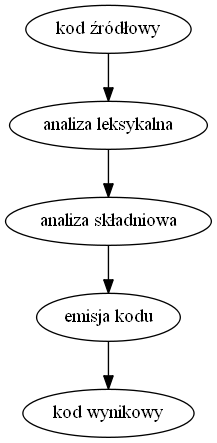
\includegraphics[width=5cm]{basic-compiler-flow}
    \caption{Podstawowy schemat budowy kompilatora}
    \label{basic_compiler_flow}
\end{figure}

Na rysunku \ref{basic_compiler_flow} przedstawiony jest uproszczony schemat budowy kompilatora.
W kompilatorach ''produkcyjnych'' (np. GCC, Clang, czy ICC) tych faz jest więcej -- przede wszystkim etap
emisji kodu jest dużo bardziej rozbudowany, oraz dochodzą etapy analizy semantycznej (czy program ma sens) czy
optymalizacji (prób takiego przekształcenia kodu programu żeby przy zachowaniu znaczenia działał wydajniej).

Kompilator języka ViuAct dostarczany jako element tej pracy inżynierskiej jest pozbawiony etapów
analizy semantycznej oraz optymalizacji. Analiza semantyczna (oraz weryfikacja typów i wykrywanie błędów na
etapie kompilacji) jest oddelegowana do assemblera dostarczanego przez platformę. Optymalizacja jest
całkowicie pominięta gdyż jest to temat niezwykle rozległy; implementacja i doszlifowanie algorytmów
optymalizujących kod jest sama w sobie materiałem wystarczającym na napisanie osobnej pracy inżynierskiej.

Architektura kompilatora języka ViuAct jest dokładniej opisana w rozdziale
\ref{architektura_kompilatora_viuact} (\nameref{architektura_kompilatora_viuact}) na
stronie \pageref{architektura_kompilatora_viuact}.
Sposób działania kompilatora jest opisany w rozdziale \ref{opis_etapow_kompilacji}
(\nameref{opis_etapow_kompilacji}) na stronie \pageref{opis_etapow_kompilacji}.
Omówienie interakcji kompilatora języka ViuAct z narzędziami dostarczanymi przez platformę Viua VM znajduje
się w rozdziale \ref{lang_architektura_systemu} (\nameref{lang_architektura_systemu}) na stronie
\pageref{lang_architektura_systemu}.

Oprócz kompilatora (rozdział \ref{opis_kompilatora} na stronie \pageref{opis_kompilatora}) dostarczany jest
również ''program łączący'' (rozdział \ref{opis_linkera} na stronie \pageref{opis_linkera}) dokonujący
automatycznego połączenia wymaganych modułów w gotowy plik wykonywalny.

\newpage

\subsection{Architektura systemu}
\label{lang_architektura_systemu}

Rysunek \ref{schemat_interakcji_viuact_z_viuavm} (''\nameref{schemat_interakcji_viuact_z_viuavm}'') prezentuje
schemat interakcji jakie zachodzą w całym systemie od momentu wczytania pliku źródłowego przez kompilator do
uruchomienia programu przez jądro Viua VM.

Ostatnią fazą jaką zajmuje się kompilator języka ViuAct dostarczany jako element tej pracy inżynierskiej jest
emisja kodu (''Assembly code emission''), której wynikiem jest plik z kodem źródłowym w języku assemblera Viua
VM (''\texttt{hello\_world.asm}'' na rysunku). Rozdział \ref{architektura_kompilatora_viuact}
(\nameref{architektura_kompilatora_viuact}) dokładniej opisuje działanie samego kompilatora.

\begin{figure}[!htp]
    \centering
    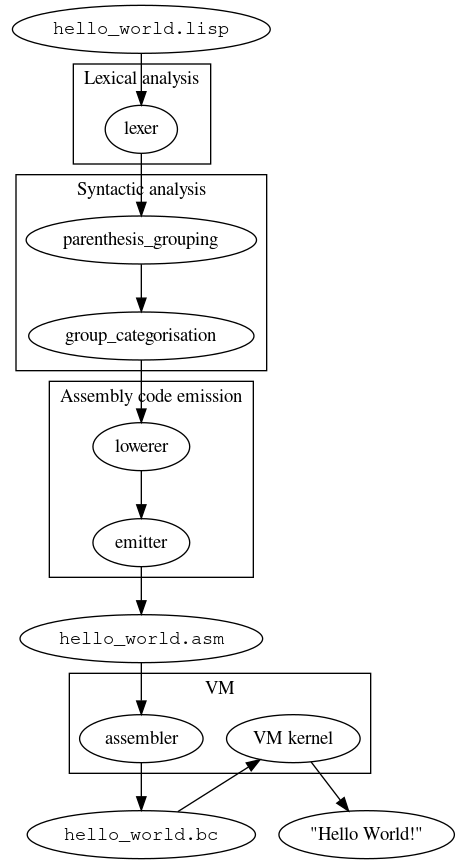
\includegraphics[width=9cm]{viuact-pipeline}
    \caption{Interakcje: od pliku źródłowego do działającego programu}
    \label{schemat_interakcji_viuact_z_viuavm}
\end{figure}

Zakres pracy inżynierskiej obejmuje wygenerowanie pliku zawierającego poprawny kod w języku
assemblera Viua VM oraz plików pomocniczych (zadanie kompilatora), oraz takim pokierowaniu
narzędziami dostarczanymi przez platformę, żeby wyemitowały one plik wykonywalny bądź bibliotekę (zadanie
''programu łączącego''). Zakładamy, że narzędzia dostarczane przez platformę działają poprawnie.

Pliki pomocnicze są wymagane przez ''program łączący'' (opisany w rozdziale \ref{opis_linkera} na stronie
\pageref{opis_linkera}). Ich dokładniejsze opisy znajdują się w rozdziałach
''\nameref{pliki_interfejsow_modulow}'' na stronie \pageref{pliki_interfejsow_modulow} i
''\nameref{pliki_zaleznosci_modulow}'' na stronie \pageref{pliki_zaleznosci_modulow}

\subsection{Dekompozycja systemu na podsystemy}
\label{architektura_kompilatora_viuact}

Język ViuAct jest implementowany przez dwa programy:

\begin{enumerate}
    \item \textbf{kompilator} - który przetwarza kod źródłowy w języku ViuAct na kod źródłowy w języku
        assemblera Viua VM
    \item \textbf{linker} - który na podstawie wyników pracy kompilatora tworzy pliki wykonywalne, które
        mogą być uruchomione na jądrze Viua VM
\end{enumerate}

Większość pracy w tym układzie wykonuje kompilator, opisany w rozdziale \ref{opis_kompilatora} na stronie
\pageref{opis_kompilatora}. Generuje on pliki zawierające kod źródłowy w języku assemblera gotowe do
przetworzenia przez assembler Viua VM na formę binarną, oraz pliki pomocnicze.

Z plików pomocniczych korzysta zarówno sam kompilator (do określenia interfejsów modułów importowanych przez
aktualnie kompilowany moduł), ale też linker -- do określenia jakie moduły powinny być dołączone do aktualnie
emitowanego pliku wykonywalnego, aby zapewnić dostępność wszystkich wymaganych funkcji. Linker jest dokładniej
opisany w rozdziale \ref{opis_linkera} na stronie \pageref{opis_linkera}.

\subsubsection{Kompilator -- \texttt{viuact-cc}}
\label{opis_kompilatora}

Kompilator składa się z kilku podsystemów, zgodnie z
przedstawieniem na rysunku \ref{ogolny_schemat_kompilatora_viuact}.

\begin{figure}[!htp]
    \centering
    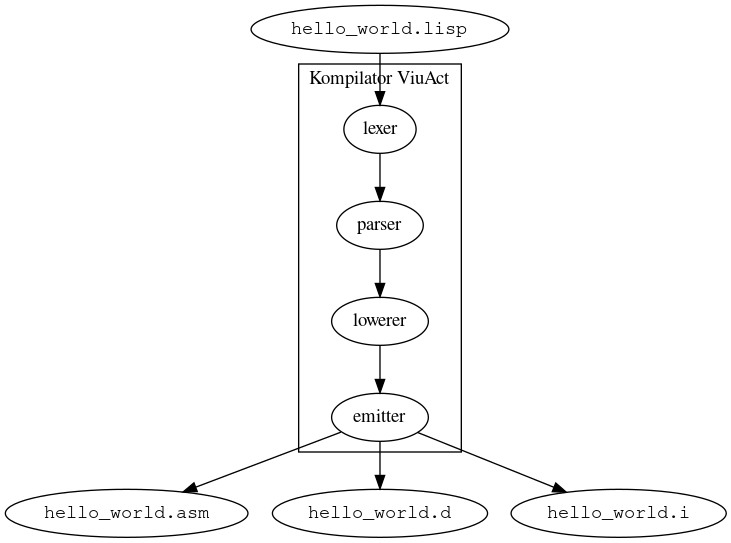
\includegraphics[width=10cm]{viuact-ogolny-schemat-kompilatora}
    \caption{Podział kompilatora na podsystemy}
    \label{ogolny_schemat_kompilatora_viuact}
\end{figure}

Każdy podsystem implementuje jedną z faz kompilacji:

\begin{enumerate}
    \item \textbf{lexer} dokonuje analizy leksykalnej wczytanego pliku źródłowego, dzieląc go na listę tokenów
    \item \textbf{parser} dokonuje analizy składniowej łącząc tokeny w grupy reprezentujące większe
        konstrukcje językowe
    \item \textbf{lowerer} mapuje grupy wyprodukowane przez \emph{parser} do odpowiednich funkcji
        \emph{emittera}; jest to dość banalny etap, ale upraszcza budowę kompilatora
    \item \textbf{emitter} tłumaczy konstrukcje językowe ViuAct na równoznaczne konstrukcje w języku
        assemblera Viua VM
\end{enumerate}

Różnica między podsystemami \emph{lowerer} i \emph{emitter} może być niejasna. Oba biorą udział w emisji
kodu wynikowego, ale \emph{lowerer} bezpośrednio zajmuje się tylko modułami i funkcjami, natomiast
\emph{emitter} implementuje emisję pojedynczych wyrażeń języka ViuAct -- przypisań \texttt{let}, konstrukcji
warunkowych \texttt{if}, wywołań funkcji, itd.

Proces kompilacji dokłaniej opisany jest w rozdziale \ref{opis_etapow_kompilacji}
(\nameref{opis_etapow_kompilacji}) na stronie \pageref{opis_etapow_kompilacji}.

\subsubsection{Program łączący -- \texttt{viuact-opt}}
\label{opis_linkera}

Program łączący (tzw. ''\emph{linker}'') zajmuje się finalną fazę ''kompilacji''.
Jest to stwierdzenie o tyle trafne, co niepoprawne. Zazwyczaj jednak nie ma to znaczenia, ponieważ zarówno
linker jak i kompilator jest ukrywany przed programistą. Popularne ''kompilatory'' jak np \emph{\texttt{g++}}
z GCC to tak naprawdę ''drivery''; wywołanie polecenia \emph{\texttt{g++}} powoduje wywołanie zarówno
kompilatora (\emph{\texttt{cc1}}), assemblera (\emph{\texttt{as}}), jak i linkera (\emph{\texttt{ld}}) w taki
sposób aby na wyjściu uzyskać oczekiwany wynik, czyli na przykład plik wykonywalny w formacie
ELF \emph{\texttt{a.out}}.

W przypadku kompilatora ViuAct proces ten wygląda podobnie, ale nie jest aż tak zautomatyzowany.
Rolę ''drivera'' pełni programista, który jest odpowiedzialny za wywołanie zarówno kompilatora jak i linkera.
Przykładowo:

\begin{lstlisting}
viuact-cc --mode exec ./hello_world.lisp
viuact-opt ./build/_default/hello_world.asm
\end{lstlisting}

Program łączący przeprowadzi proces asemblacji pliku podanego na wejściu, oraz dołączy do niego wszelkie
wymagane moduły. Zarówno asemblacja jak i łączenie będa przeprowadzone przez narzędzie dostarczane przez
platformę Viua VM -- \texttt{viuact-opt} zajmuje się jedynie wygenerowaniem odpowiednich poleceń dla tego
narzędzia.

Informacja o tym jakie moduły muszą zostać dołączone jest tworzona w oparciu o pliki zależności (opisane w
rozdziale \nameref{pliki_zaleznosci_modulow} na stronie \pageref{pliki_zaleznosci_modulow}).
Dla uproszczenia projektu program łączący nie zbiera informacji o zależnościach rekurencyjnie.

Po zebraniu informacji o zależnościach program łączący dokonuje asemblacji wszystkich modułów, od których
zależy kompilowany moduł główny. Następnie asembluje moduł główny i łączy wszystkie wyemitowane modułu
bytecode'u w gotowy plik wykonywalny.

\subsection{Przebieg procesu kompilacji}
\label{opis_etapow_kompilacji}

Ten rozdział zawiera dokładny opis procesu kompilacji, od momentu wczytania pliku z kodem źródłowym w języku
ViuAct do momentu wyemitowania kodu wynikowego w języku assemblera Viua VM. Kompilator jest wywoływany
poleceniem \texttt{viuact-cc} z opcją \texttt{-}\texttt{-mode} określającą czy kompilowany jest moduł wykonywalny
(\texttt{exec}) czy moduł biblioteki (\texttt{module}):

\begin{lstlisting}
viuact-cc --mode ( 'exec' | 'module' ) file.lisp
\end{lstlisting}

\subsubsection{Wczytanie pliku źródłowego}

Kompilator wczytuje do pamięci cały plik źródłowy jako pojedynczy string.

\subsubsection{Analiza leksykalna}

Lexer patrzy na wczytany kod źródłowy i do pierwszego nieprzeanalizowanego znaku (czyli na początku analizy do
znaku na indeksie 0) próbuje przypasować wzorzec określający jaki token znajduje się na tej pozycji. Po udanym
przypasowaniu pozycja, która będzie rozpatrywana przez lexer jest przesuwana o tyle znaków ile wynosi długość
wygenerowanego tokenu i lexer rozpoczyna pracę od nowa. Ten proces trwa do momentu aż cały string wejściowy
nie zostanie przeanalizowany, albo odrzucony jako nieprawidłowy.

Algorytm przypasowania jest banalny. Lexer dysponuje listą wzorców (określonych przez wyrażenia regularne),
które określają jak wygląda każdy możliwy token w języku. Lexer po kolei próbuje przypasować każdy wzorzec z
listy i kończy na pierwszym trafieniu. Jeśli żaden wzorzec nie może zostać przypisany lexer odrzuca kod
źródłowy jako nieprawidłowy.

Wzorce są uszeregowane w taki sposób żeby nie była możliwa pomyłka i
na przykład przypasowanie początku nazwy zmiennej \texttt{letter} jako słowa kluczowego \texttt{let}.

\subsubsection{Analiza składniowa}
\label{opis_etapow_kompilacji_analiza_skladniowa}

Składnia języka została zaprojektowana w taki sposób aby analiza składniowa mogła być uproszczona do maksimum
i prosta w implementaji.

\paragraph{Grupowanie nawiasów}

W pierwszej fazie analizy składniowej tokeny grupowane są wegług nawiasów okrągłych, przy czym grupowanie jest
rekurencyjne (jeśli jakaś grupa zawiera podgrupę w nawiasach to zagnieżdżona grupa będzie widoczna jako
pojedynczy element w grupie zewnętrznej).
Dla przykładu:

\begin{lstlisting}
(let x (frobnicate 42))
\end{lstlisting}

będzie zgrupowane w następujący sposób:

\begin{lstlisting}
[ "let"; "x"; [ "frobnicate"; "42" ] ]
\end{lstlisting}

\paragraph{Grupowanie id}

Kolejnym etapem jest grupowanie id. Id jest nazwą składającą się z kilku członów, na przykład
\texttt{Std.Posix.Network.socket} składa się z 7 tokenów: trzech \emph{nazw modułów} (\texttt{Str},
\texttt{Posix}, i \texttt{Network}), trzech \emph{operatorów dostępu} (kropek), i jednej \emph{nazwy}
(\texttt{socket}).
Taka grupa zostanie na tym etapie zredukowana do pojedynczego elementu.

\paragraph{Oznczanie wyrażeń złożonych}

Wyrażenia złożone składają się z kilku wyrażeń (prostych bądź złożonych). Z uwagi na fakt, że formą pośrednią
wykorzystywaną na etapie grupowania są listy tokenów takie wyrażenie byłoby nieodróżnialne od listy
reprezentującej wywołanie funkcji. Dlatego na etapie analizy składniowej do list reprezentujących wyrażenia
złożone dodawany jest specjalny token-fantom. Dzięki temu zostaje zachowana właściwość umożliwiająca szybkie
klasyfikowanie grup. Dla przykładu:

\begin{lstlisting}
(let x { ... })
\end{lstlisting}

będzie zgrupowane w następujący sposób:

\begin{lstlisting}
[ "let"; "x"; [ Compound_expression_marker; ... ] ]
\end{lstlisting}

\paragraph{Klasyfikacja grup}

Ostatnim etapem analizy składniowej jest klasyfikacja grup. W większości przypadków do klasyfikacji listy
tokenów do grupy reprezentującej konkretną konstrukcję językową wystarczy spojrzeć na pierwszy token na
liście. W niektórych przypadkach algorytm musi się posiłkować długością listy.

Dla przykładu:

\begin{lstlisting}
[ "let"; "x";          ... ]        -> let-binding
[ "let"; "x"; [ ... ]; ... ]        -> function-definition
[ ... ]                             -> function-call
[ "actor"; ... ]                    -> actor-call
[ Compound_expression_marker; ... ] -> compound-call
\end{lstlisting}

Różnicą między definicją zmiennej (\texttt{let-binding}), a definicją funkcji (\texttt{function-definition})
jest długość listy - definicja zmiennej zawiera trzy elementy (słowo kluczowe \texttt{let}, nazwę, i
wyrażenie), a definicja funkcji cztery elementy (słowo kluczowe \texttt{let}, nazwę, listę parametrów
formalnych, i wyrażenie).

\subsubsection{Emisja modułów}

W następnej kolejności emitowane są wszystkie moduły zagnieżdżone w aktualnie kompilowanym module, przy czym
ten etap postępuje rekurencyjnie. Moduły zagnieżdżone musżą być wyemitowane przed modułem głównym, aby
kompilator miał dostęp do ich plików interfejsów i umożliwić ich importowanie.

\subsubsection{Analiza importu modułów}

Kolejnym krokiem jest analiza modułów importowanych przez aktualnie kompilowany moduł i wczytanie ich
interfejsów.

\subsubsection{Emisja kodu wynikowego}
\label{opis_etapow_kompilacji_emisja_kodu_wynikowego}

Na końcu następuje emisja kodu wynikowego w języku assemblera Viua VM. Ten etap jest wykonywany osobno dla
każdej funkcji zdefiniowanej w kompilowanym module.

\paragraph{Redukcja poziomu wyrażeń}

Najpierw następuje redukcja poziomu wyrażeń. Tym etapem zajmuje się \emph{lowerer}. Jest to mechaniczny proces
mapujący sklasyfikowane grupy reprezentujące konretne konstrukcje językowe do funkcji udostępnianych przez
\emph{emitter}, opakowanie wyniku w sposób jakiego wymagają zasady języka assemblera Viua VM, oraz
serializacja wyników do stringów.

\paragraph{Emisja instrukcji języka assemblera}

Emisja instrukcji języka assemblera jest wykonywana per-wyrażenie. Ten etap przeplata się z redukcją poziomu
wyrażeń i jest implementowany przez \emph{emitter}. \emph{Emitter} emituje sekwencje instrukcji języka
assemblera Viua VM odpowiadające zadanym konstrukcjom językowym ViuAct.

Dla przykładu \texttt{(let x 42)} zostanie wyemitowane jako pojedyncza instrukcja: \texttt{integer \%x local
42}.  Natomiast \texttt{(Some\_module.frobnicate 42)} zostanie wyemitowane jako sekwencja instrukcji:

\begin{lstlisting}
integer %3 local 42
frame %1 arguments
copy %0 arguments %3 local
call void Some_module::frobnicate/1
\end{lstlisting}

\subsubsection{Zapis pliku \texttt{.asm}}

Dla każdego wyemitowanego modułu kompilator zapisze plik \texttt{\emph{nazwa\_modulu}.asm} zawierający kod
wynikowy w języku assemblera Viua VM.

\subsubsection{Zapis pliku \texttt{.i}}

Dla każdego wyemitowanego modułu biblioteki kompilator zapisze plik \texttt{\emph{nazwa\_modulu}.i}
zawierający definicję interfejsu tego modułu. Pliki interfejsów są opisane w rozdziale
\nameref{pliki_interfejsow_modulow} na stronie \pageref{pliki_interfejsow_modulow}.

\subsubsection{Zapis pliku \texttt{.d}}

Dla każdego wyemitowanego modułu kompilator zapisze plik \texttt{\emph{nazwa\_modulu}.d}
zawierający definicję zależności tego modułu. Pliki zależności są opisane w rozdziale
\nameref{pliki_zaleznosci_modulow} na stronie \pageref{pliki_zaleznosci_modulow}.
